\documentclass{article} % For LaTeX2e
\usepackage{nips15submit_e,times}
\usepackage{hyperref}
\usepackage{url}
\usepackage{times}
\usepackage{relsize}
\usepackage{xcolor,colortbl}
\usepackage{multirow}
\usepackage{epsfig}
\usepackage{graphicx}
\usepackage{wrapfig}
\usepackage{bbm}
\usepackage[labelfont=bf]{caption}
\usepackage{tabularx}
\usepackage{amsmath}
\usepackage{amssymb}
%\documentstyle[nips14submit_09,times,art10]{article} % For LaTeX 2.09


\title{You Only Look Once: \\
Unified, Real-Time Object Detection}


\author{Joseph Red\$\\
University of Washington\\
\texttt{pjreddie@cs.washington.edu}
% For a paper whose authors are all at the same institution,
% omit the following lines up until the closing ``}''.
% Additional authors and addresses can be added with ``\and'',
% just like the second author.
% To save space, use either the email address or home page, not both
\and
Santosh Divvala\\
Allen Institute for Artificial Intelligence\\
\texttt{santoshd@allenai.org}
\and
Ross Girshick\\
Microsoft Research\\
\texttt{rbg@microsoft.com}
\and
Ali Farhadi\\
University of Washington\\
\texttt{ali@cs.washington.edu}
}

% The \author macro works with any number of authors. There are two commands
% used to separate the names and addresses of multiple authors: \And and \AND.
%
% Using \And between authors leaves it to \LaTeX{} to determine where to break
% the lines. Using \AND forces a linebreak at that point. So, if \LaTeX{}
% puts 3 of 4 authors names on the first line, and the last on the second
% line, try using \AND instead of \And before the third author name.

\newcommand{\fix}{\marginpar{FIX}}
\newcommand{\new}{\marginpar{NEW}}

%\nipsfinalcopy % Uncomment for camera-ready version

\begin{document}


\maketitle

\begin{abstract}
We present YOLO, a unified pipeline for object detection. Prior work on object detection repurposes classifiers to perform detection. Instead, we frame object detection as a regression problem to spatially separated bounding boxes and associated class probabilities. A single neural network predicts bounding boxes and class probabilities directly from full images in one evaluation. Since the whole detection pipeline is a single network, it can be optimized end-to-end directly on detection performance. Our unified architecture is also extremely fast; YOLO processes images in real-time at 45 frames per second, hundreds to thousands of times faster than existing detection systems. Our system uses global image context to detect and localize objects, making it less prone to background errors than top detection systems like R-CNN. By itself, YOLO detects objects at unprecedented speeds with moderate accuracy. When used in combination with state-of-the-art detectors, YOLO boosts performance by 2-3\% points mAP.
\end{abstract}

\section{Introduction}

Humans glance at an image and instantly know what objects are in the image, where they are, and how they interact. The human visual system is fast and accurate, allowing us to perform complex tasks like driving or grocery shopping with little conscious thought. Fast, accurate, algorithms for object detection would allow computers to drive cars in any weather without specialized sensors, enable assistive devices to convey real-time scene information to human users, and unlock the potential for general purpose, responsive robotic systems.

Convolutional neural networks (CNNs) achieve impressive performance on classification tasks at real-time speeds \cite{DBLP:journals/corr/HeZR015}. Yet top object detection systems like R-CNN take seconds to process individual images and hallucinate objects in background noise. We believe these shortcomings result from how these systems approach object detection.

Current detection systems repurpose classifiers to perform detection. To detect an object these systems take a classifier for that object and evaluate it at various locations and scales in a test image. Systems like deformable parts models (DPM) use a sliding window approach where the classifier is run at evenly spaced locations over the entire image \cite{lsvm-pami}. More recent approaches like R-CNN use region proposal methods to first generate potential bounding boxes in an image and then run a classifier on these proposed boxes. After classification, post-processing is used to refine the bounding box, eliminate duplicate detections, and rescore the box based on other objects in the scene \cite{girshick2014rich}.

\begin{figure}[t]
\begin{center}
        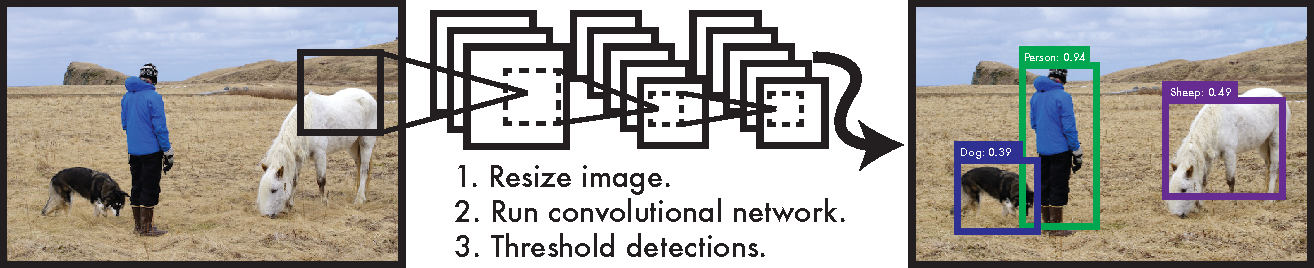
\includegraphics[width=\linewidth]{system2}
\end{center}
   \caption{\textbf{The YOLO Detection System.} Processing images with YOLO is simple and straightforward. Our system (1) resizes the input image to $448 \times 448$, (2) runs a single convolutional network on the image, and (3) thresholds the resulting detections by the model's confidence.}
\label{system}
\end{figure}

These region proposal techniques typically generate a few thousand potential boxes per image. Selective Search, the most common region proposal method, takes 1-2 seconds per image to generate these boxes \cite{uijlings2013selective}. The classifier then takes additional time to evaluate the proposals. The best performing systems require 2-40 seconds per image and even those optimized for speed do not achieve real-time performance. Additionally, even a highly accurate classifier will produce false positives when faced with so many proposals. When viewed out of context, small sections of background can resemble actual objects, causing detection errors.

Finally, these detection pipelines rely on independent techniques at every stage that cannot be optimized jointly. A typical pipeline uses Selective Search for region proposals, a convolutional network for feature extraction, a collection of one-versus-all SVMs for classification, non-maximal suppression to reduce duplicates, and a linear model to adjust the final bounding box coordinates. Selective Search tries to maximize recall while the SVMs optimize for single class accuracy and the linear model learns from localization error.

Our system is refreshingly simple, see Figure \ref{system}. A single convolutional network simultaneously predicts multiple bounding boxes and class probabilities for those boxes. We train our network on full images and directly optimize detection performance. Context matters in object detection. Our network uses global image features to predict detections which drastically reduces its errors from background detections. At test time, a single network evalution of the full image produces detections of multiple objects in multiple categories without any pre or post-processing.

Our training and testing code are open source and available online at [redacted]. A variety of pre-trained models are also available to download.

\section{Unified Detection}

We unify the separate components of object detection into a single neural network. Using our system, you only look once (YOLO) at an image to predict what objects are present and where they are. Our network uses features from the entire image to predict each bounding box. It also predicts all bounding boxes for an image simultaneously. This means our network reasons globally about the full image and all the objects in the image. The YOLO design enables end-to-end training and real-time speeds while maintaining high average precision.

\begin{figure}[h]
\begin{center}
        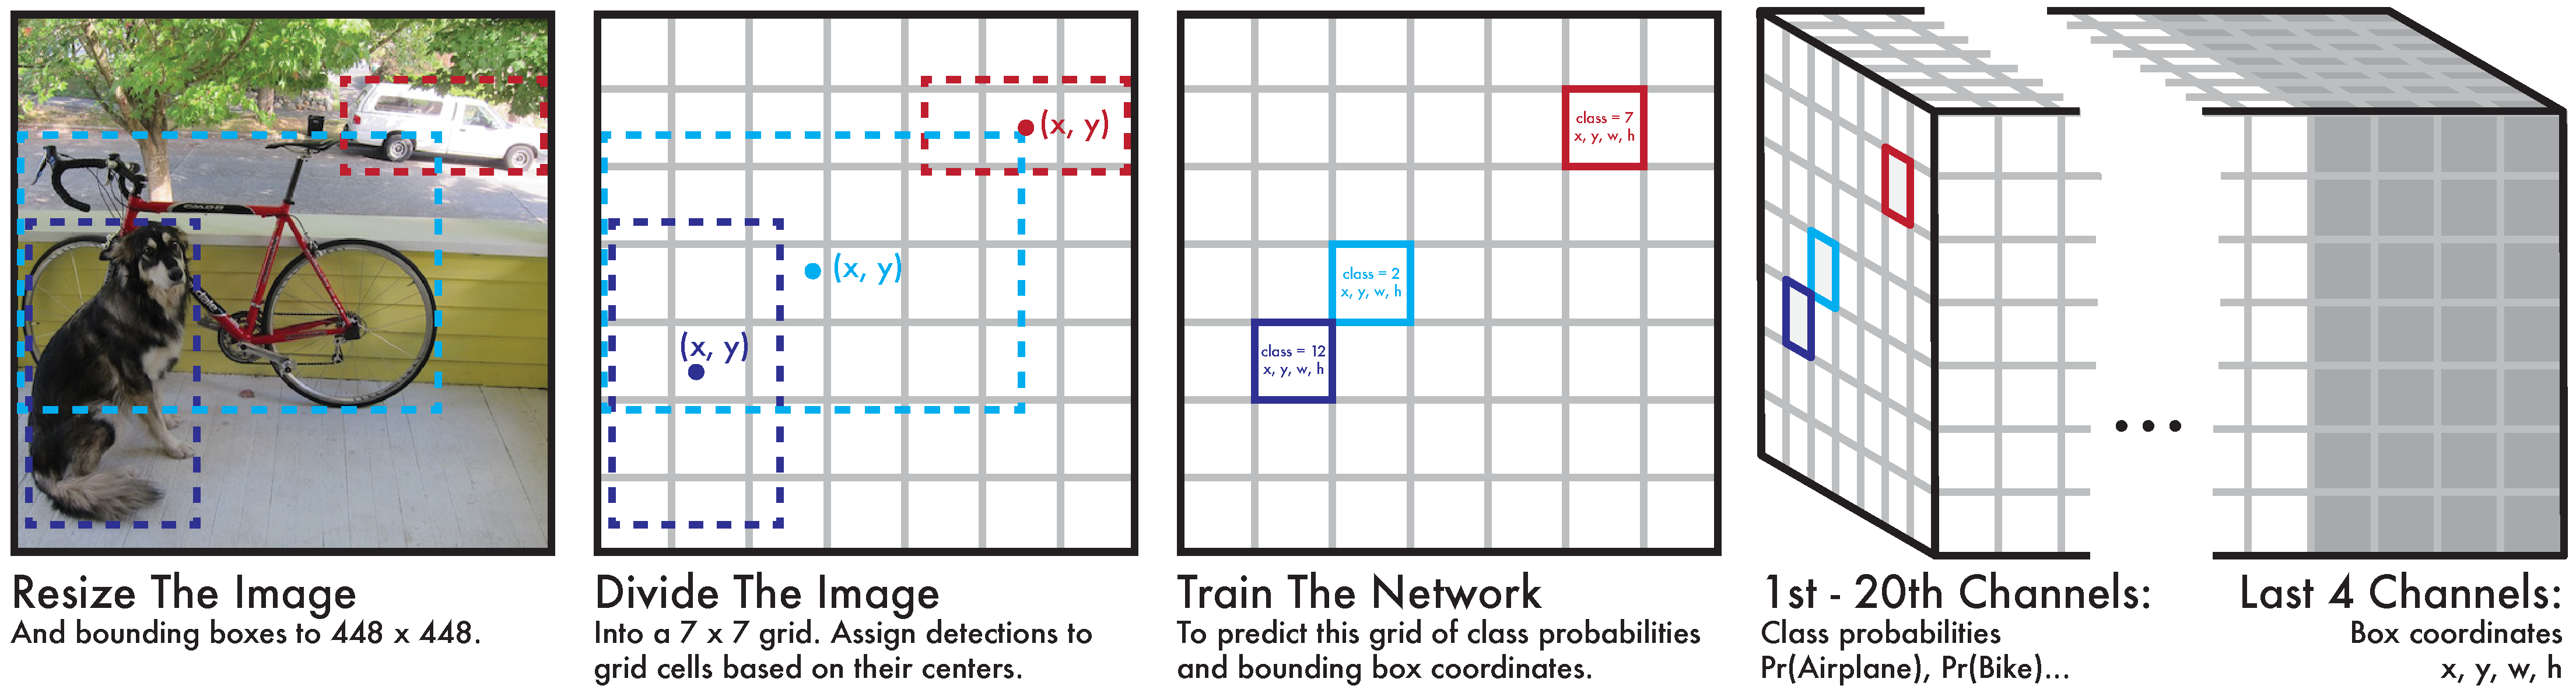
\includegraphics[width=\linewidth]{full}
\end{center}
   \caption{\textbf{The Model.} Our system models detection as a regression problem to a $7 \times 7 \times 24$ tensor. This tensor encodes bounding boxes and class probabilities for all objects in the image.}
\label{model}
\end{figure}

\subsection{Design}

Our system divides the input image into a $7 \times 7$ grid. If the center of an object falls into a grid cell, that grid cell is responsible for detecting that object. Each grid cell predicts a bounding box and class probabilities associated with that bounding box, see Figure \ref{model}.

We implement this model as a convolutional neural network and evaluate it on the \textsc{Pascal} VOC detection dataset \cite{Everingham15}. The initial convolutional layers of the network extract features from the image while the fully connected layers predict the output probabilities and coordinates.

Our network architecture is inspired by the GoogLeNet model for image classification \cite{DBLP:journals/corr/SzegedyLJSRAEVR14}. Our nework has 24 convolutional layers followed by 2 fully connected layers. However, instead of the inception modules used by GoogLeNet we simply use $1 \times 1$ reduction layers followed by $3 \times 3$ convolutional layers, similar to Lin et al \cite{DBLP:journals/corr/LinCY13}. We also replace maxpooling layers with strided convolutions. The full network is shown in Figure \ref{net}.

The final output of our network is a $7 \times 7$ grid of predictions. Each grid cell predicts 20 conditional class probabilities, and 4 bounding box coordinates.

   \begin{figure}[h]
      \centering
        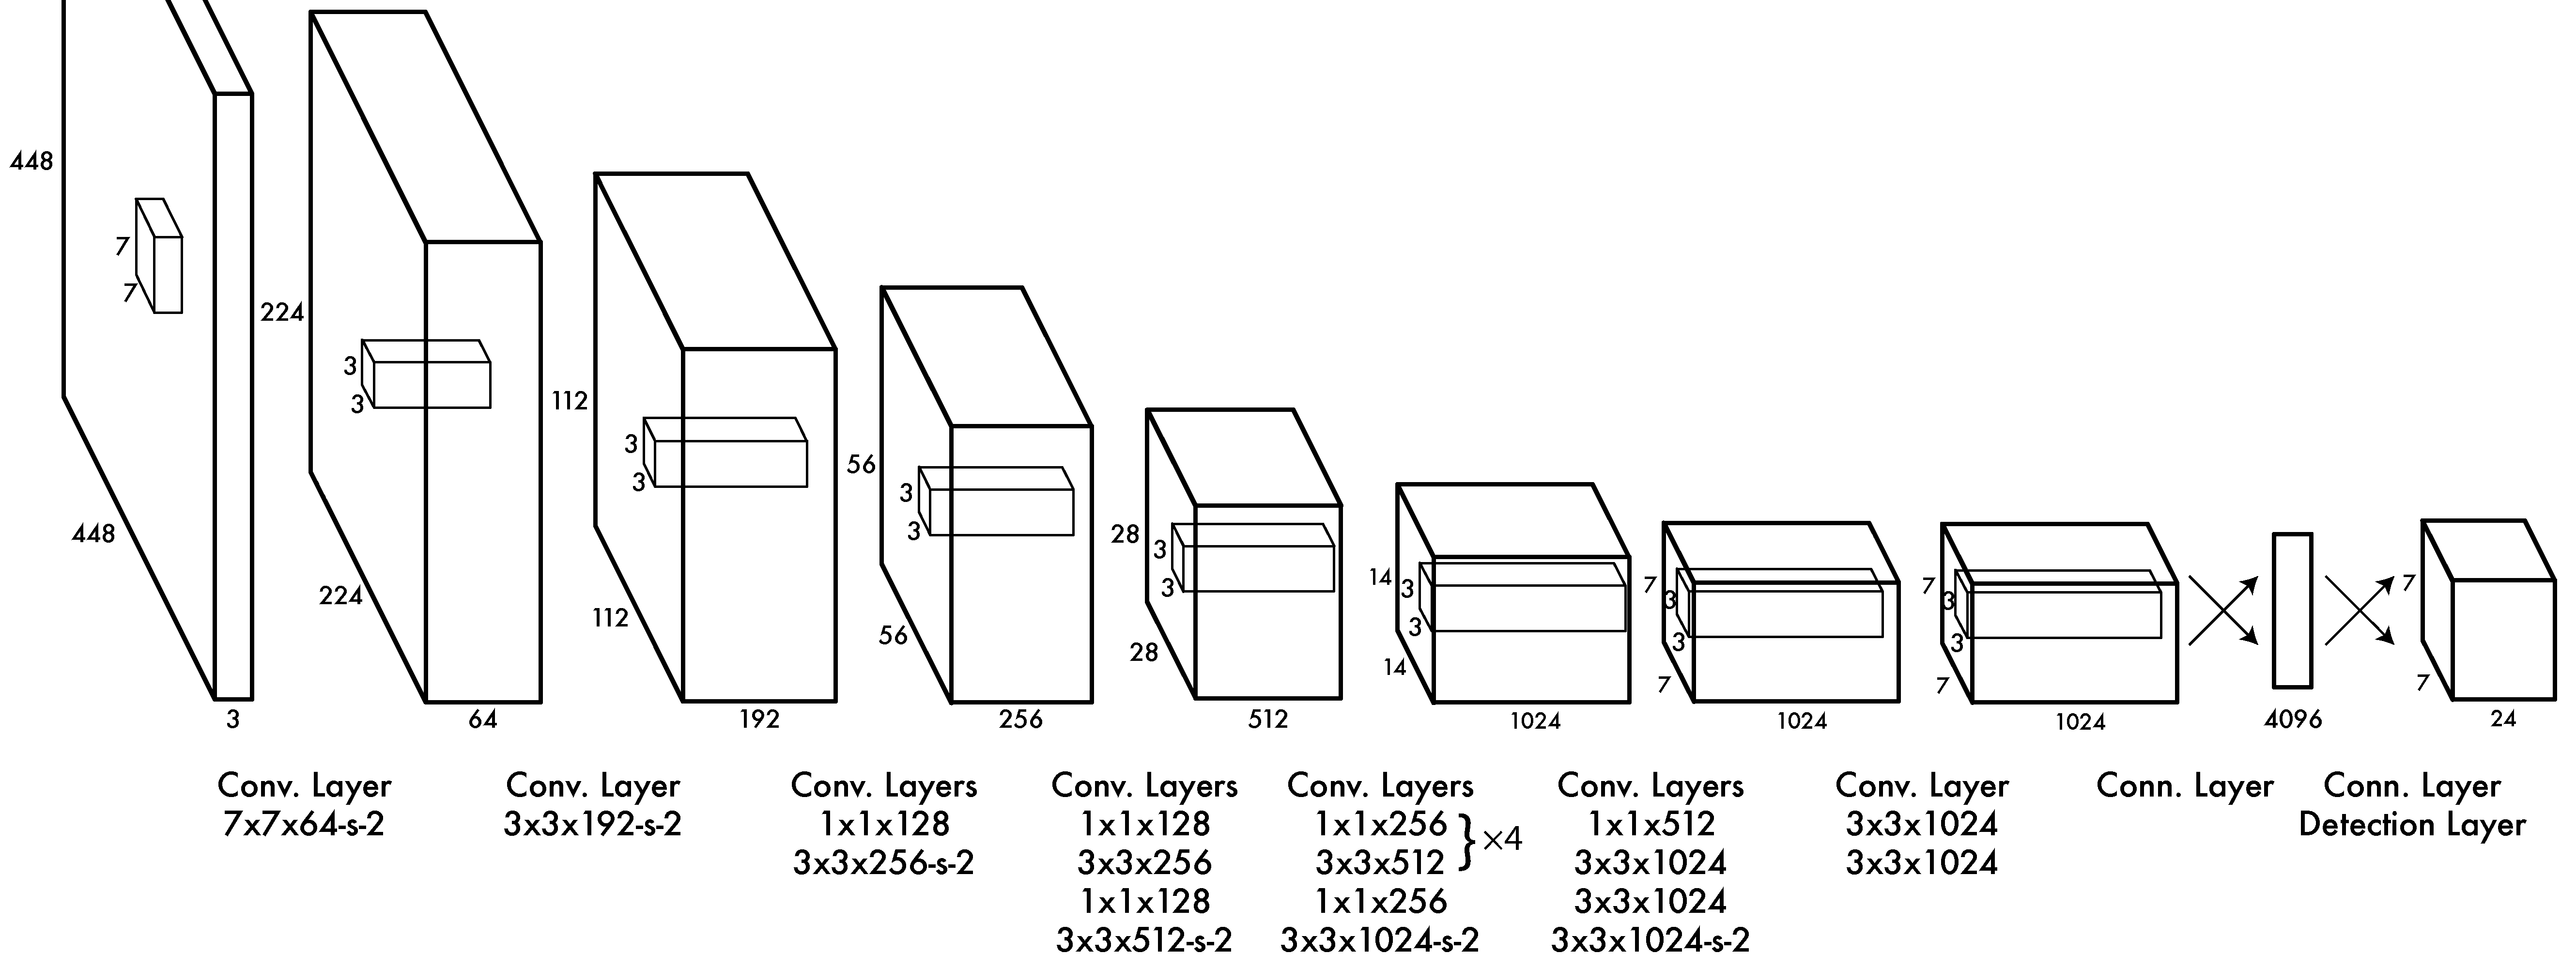
\includegraphics[width=\linewidth]{detectnet2}
      \caption{\textbf{The Architecture.} Our detection network has 24 convolutional layers followed by 2 fully connected layers. The network uses strided convolutional layers to downsample the feature space instead of maxpooling layers. Alternating $1 \times 1$ convolutional layers reduce the features space from preceeding layers. We pretrain the convolutional layers on the ImageNet classification task at half the resolution ($224 \times 224$ input image) and then double the resolution for detection.}
      \label{net}
   \end{figure}

\subsection{Training}

   \begin{figure}[t]
      \centering
        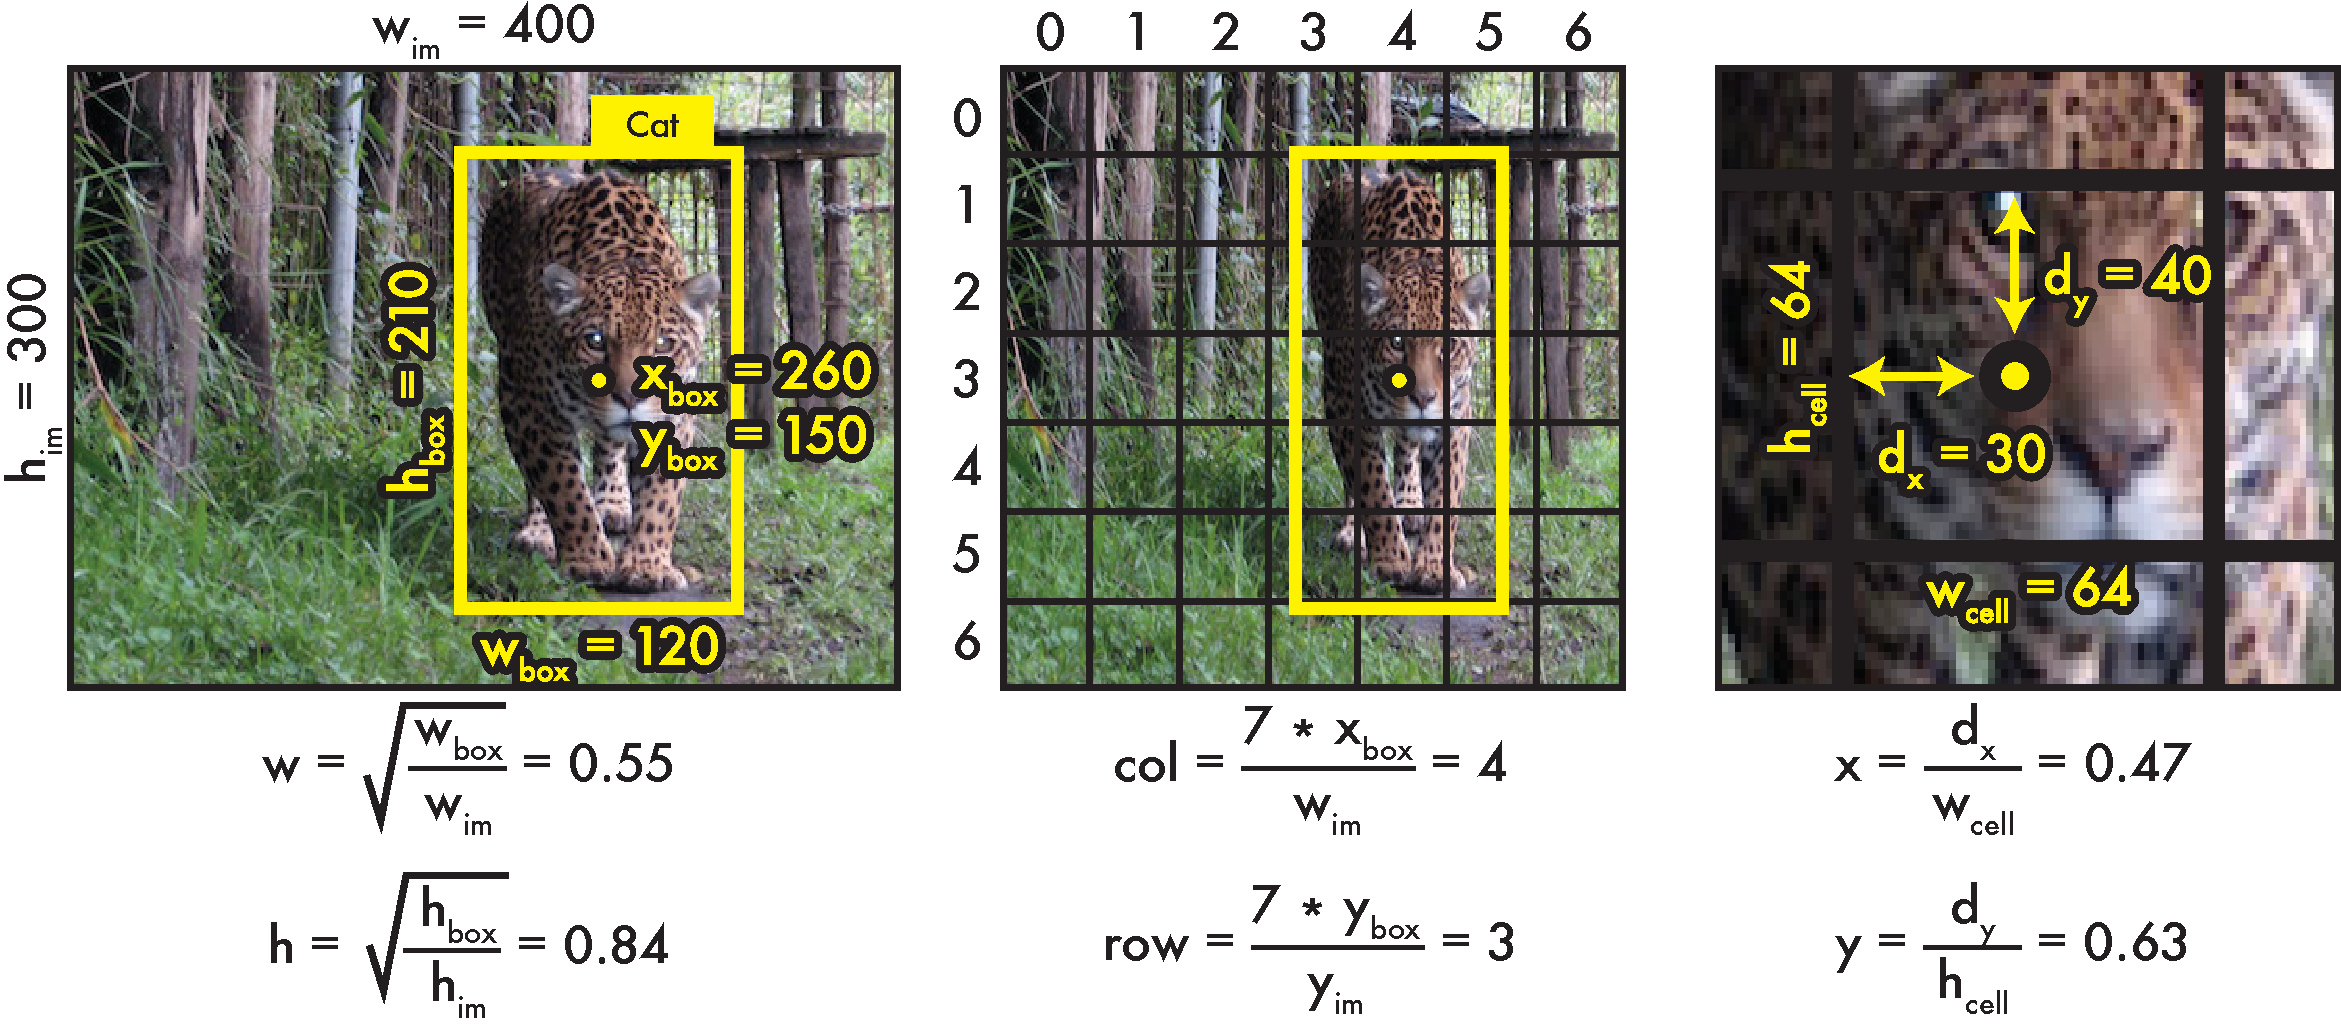
\includegraphics[width=.8\linewidth]{transform}
      \caption{\textbf{The Coordinate System.} This image shows an example transformation from bounding box coordinates to the coordinates used by our output layer. Left: We normalize width and height by the width and height of the image. Middle: We find the appropriate grid cell based on the center of the bounding box. Right: We calculate the center coordinate offsets relative to the position of the grid cell.}
      \label{transform}
   \end{figure}

We pretrain our convolutional layers on the ImageNet 1000-class competition dataset \cite{ILSVRC15}. For pretraining we use the first 20 convolutional layers from Figure \ref{net} followed by a maxpooling layer and two fully connected layers. We train this network for approximately a week and achieve a top-5 accuracy of 86\% on the ImageNet 2012 validation set.

We then adapt the model to perform detection. Ren et al. show that adding both convolutional and connected layers to pretrained networks can benefit performance \cite{DBLP:journals/corr/RenHGZ015}. Following their example, we add four convolutional layers and two fully connected layers with randomly initialized weights. Detection often requires fine-grained visual information so we increase the input resolution of the network from $224 \times 224$ to $448 \times 448$.

Our final layer predicts both class probabilities and bounding box coordinates. We normalize the bounding box width and height by the image width and height so that they fall between 0 and 1. We parameterize the bounding box $x$ and $y$ coordinates to be offsets of a particular grid cell location so they are also bounded between 0 and 1. We use a logistic activation function to reflect these constraints on the final layer. All other layers use the following leaky rectified linear activation:

\begin{equation}
\phi(x) =
\begin{cases}
    1.1x, & \text{if } x > 0\\
    .1x, & \text{otherwise}
    \end{cases}
\end{equation}

We optimize for sum-squared error in the output of our model. We use sum-squared error because it is easy to optimize, however it does not perfectly align with our goal of maximizing average precision. It weights localization error equally with classification error which may not be ideal. To remedy this, we use a scaling factor $\lambda$ to adjust the weight given to error from coordinate predictions versus error from class probabilities. In our final model we use the scaling factor $\lambda = 4$.

Sum-squared error also equally weights errors in large boxes and small boxes. Our error metric should reflect that small deviations in large boxes matter less than in small boxes. To partially address this we predict the square root of the bounding box width and height instead of the width and height directly. Figure \ref{transform} shows an example transformation of a bounding box from image coordinates to the coordinates used by YOLO.

If cell $i$ predicts class probabilities $\hat{p}_i(\text{aeroplane}), \hat{p}_i(\text{bicycle})...$ and the bounding box $\hat{x}_i,\hat{y}_i, \hat{w}_i, \hat{h}_i$ then our full loss function for an example is:

\begin{equation}
\sum_{i = 0}^{48} \biggl( \lambda \mathlarger{\mathbbm{1}}_i^{\text{obj}}\bigl((x_i - \hat{x}_i)^2 + (y_i - \hat{y}_i)^2 + (\sqrt{w_i} - \sqrt{\hat{w}_i})^2 + (\sqrt{h_i} - \sqrt{\hat{h}_i})^2\bigr) + \sum_{c \in \text{classes}} (p_i(c) - \hat{p}_i(c))^2 \biggr)
\end{equation}

Where $\mathbbm{1}_i^{\text{obj}}$ encodes whether any object appears in cell $i$. Note that if there is no object in a cell we do not consider any loss from the bounding box coordinates predicted by that cell. In this case, there is no ground truth bounding box so we only penalize the associated probabilities with that region.

We train the network for about 120 epochs on the training and validation data sets from \textsc{Pascal} VOC 2007 and 2012 as well as the test set from 2007, a total of 21k images. Throughout training we use a batch size of 64, a momentum of $0.9$ and a decay of $0.0005$. We use two learning rates during training: $10^{-2}$ and $10^{-3}$. Training diverges if we use the higher learning rate, $10^{-2}$, from the start. We use the lower rate, $10^{-3}$, for one epoch so that the randomly initialized weights in the final layers can settle to reasonable values. Then we train with the following learning rate schedule: $10^{-2}$ for 80 epochs, and $10^{-3}$ for 40 epochs.

To avoid overfitting we use dropout and extensive data augmentation. A dropout layer with rate~=~.5 after the first connected layer prevents co-adaptation between layers \cite{hinton2012improving}. For data augmentation we introduce random scaling and translations of up to 10\% of the original image size. We also randomly adjust the exposure and saturation of the image by up to a factor of 2.

\subsubsection{Parameterizing Class Probabilities}

Each grid cell predicts class probabilities for that area of the image. There are 49 cells with a possible 20 classes each yielding 980 predicted probabilities per image. Most of these probabilities will be zero since only a few objects appear in any given image. Left unchecked, this imbalance pushes all of the probabilities to zero, leading to divergence during training.

To overcome this, we add an extra variable to each grid location, the probability that any object exists in that location regardless of class. Thus instead of 20 class probabilities we have 1 ``objectness" probability, $\Pr(\textrm{Object})$, and 20 conditional probabilities: $\Pr(\textrm{Airplane} | \textrm{Object})$, $\Pr(\textrm{Bicycle} | \textrm{Object})$, etc.

To get the unconditional probability for an object class at a given location we simply multiply the ``objectness" probability by the conditional class probability:

\begin{equation}
\Pr(\textrm{Dog}) = \Pr(\textrm{Object}) * \Pr(\textrm{Dog} | \textrm{Object})
\end{equation}

We can optimize these probabilities independently or jointly using a novel ``detection layer" in our convolutional network. During the initial stages of training we optimize them independently to improve model stability. We update the ``objectness" probabilities at every location however we only update the conditional probabilities at locations that actually contain an object. This means there are far fewer probabilities getting pushed towards zero. 

During later stages of training we optimize the unconditioned probabilities by performing the required multiplications in the network and calculating error based on the result.

\subsubsection{Predicting IOU}

Like most detection systems, our network has trouble precisely localizing small objects. While it may correctly predict that an object is present in an area of the image, if it does not predict a precise enough bounding box the detection is counted as a false positive.

We want YOLO to have some notion of uncertainty in its probability predictions. Instead of predicting 1-0 probabilities we can scale the target class probabilities by the IOU of the predicted bounding box with the ground truth box for a region. When YOLO predicts good bounding boxes it is also encouraged to predict high class probabilities. For poor bounding box predictions it learns to predict lower confidence probabilities.

We do not train to predict IOU from the beginning, only during the second stage of training. It is not necessary for good performance but it does boost our mean average precision by 3-4\%.

\subsection{Inference}

Just like in training, predicting detections for a test image only requires one network evaluation. The network predicts 49 bounding boxes per image and class probabilities for each box. YOLO is extremely fast at test time since it only requires a single network evaluation unlike classifier-based methods.

The grid design enforces spatial diversity in the bounding box predictions. Often it is clear which grid cell an object falls in to and the network only predicts one box for each object. However, some large objects or objects near the border of multiple cells can be well localized by multiple cells. Non-maximal suppression can be used to fix these multiple detections. While not critical to performance as it is for R-CNN or DPM, non-maximal suppression adds 2-3\% in mAP.

%While this limits our performance on benchmarks like \textsc{Pascal}, it also mimics how humans visually percieve objects. Humans quickly count small numbers of objects ($N \le 4$) but take significantly more time per object to count larger groups of objects \cite{piazza2002subitizing}. This suggests that the human visual system can natively handle a small number of objects but after some threshold we require additional post-processing.
\subsection{Limitations of YOLO}

YOLO imposes strong spatial constraints on bounding box predictions since each grid cell only predicts one box. This spatial constraint limits the number of nearby objects that our model can predict. If two objects fall into the same cell our model can only predict one of them. Our model struggles with small objects that appear in groups, such as flocks of birds.

Since our model learns to predict bounding boxes from data, it struggles to generalize to objects in new or unusual aspect ratios or configurations. Our model also uses relatively coarse features for predicting bounding boxes since our architecture has multiple downsampling layers from the input image.

Finally, while we train on a loss function that approximates detection performance, our loss function treats errors the same in small bounding boxes versus large bounding boxes. A small error in a large box is generally benign but a small error in a small box has a much greater effect on IOU. Our main source of error is incorrect localizations.


\section{Comparison to Other Detection Systems}

Object detection is a core problem in computer vision. Detection pipelines generally start by extracting a set of robust features from input images (Haar \cite{papageorgiou1998general}, SIFT \cite{lowe1999object}, HOG \cite{dalal2005histograms}, convolutional features \cite{donahue2013decaf}). Then, classifiers \cite{viola2001robust,lienhart2002extended,girshick2014rich,lsvm-pami} or localizers \cite{blaschko2008learning,DBLP:journals/corr/SermanetEZMFL13} are used to identify objects in the feature space. These classifiers or localizers are run either in sliding window fashion over the whole image or on some subset of regions in the image \cite{uijlings2013selective,gould2009region,zitnick2014edge}. We compare the YOLO detection system to several top detection frameworks, highlighting key similarities and differences.

\textbf{Deformable parts models.} Deformable parts models (DPM) use a sliding window approach to object detection \cite{lsvm-pami}. DPM uses a disjoint pipeline to extract static features, classify regions, predict bounding boxes for high scoring regions, etc. Our system replaces all of these disparate parts with a single convolutional neural network. The network performs feature extraction, bounding box prediction, non-maximal suppression, and contextual reasoning all concurrently. Instead of static features, the network trains the features in-line and optimizes them for the detection task. Our unified architecture leads to a faster, more accurate model than DPM.

\textbf{R-CNN.} R-CNN and its variants use region proposals instead of sliding windows to find objects in images. These systems use region proposal methods like Selective Search \cite{uijlings2013selective} to generate potential bounding boxes in an image. Instead of scanning through every region in the window, now the classifier only has to score a small subset of potential regions in an image. Good region proposal methods maintain high recall despite greatly limiting the search space. This performance comes at a cost. Selective Search, even in ``fast mode" takes about 2 seconds to propose regions for an image.

R-CNN shares many design aspects with DPM. After region proposal, R-CNN uses the same multi-stage pipeline of feature extraction (using CNNs instead of HOG), SVM scoring, non-maximal suppression, and bounding box prediction using a linear model \cite{girshick2014rich}. 

YOLO shares some similarities with R-CNN. Each grid cell proposes a potential bounding box and then scores that bounding box using convolutional features. However, our system puts spatial constraints on the grid cell proposals which helps mitigate multiple detections of the same object. Our system also proposes far fewer bounding boxes, only 49 per image compared to about 2000 from Selective Search. Finally, our system combines these individual components into a single, jointly optimized model.

\textbf{Deep MultiBox.} Unlike R-CNN, Szegedy et al. train a convolutional neural network to predict regions of interest \cite{erhan2014scalable} instead of using Selective Search. MultiBox can also perform single object detection by replacing the confidence prediction with a single class prediction. However, MultiBox cannot perform general object detection and is still just a piece in a larger detection pipeline, requiring further image patch classification. Both YOLO and MultiBox use a convolutional network to predict bounding boxes in an image but YOLO is a complete detection pipeline.

\textbf{OverFeat.} Sermanet et al. train a convolutional neural network to perform localization and adapt that localizer to perform detection \cite{DBLP:journals/corr/SermanetEZMFL13}. OverFeat efficiently performs sliding window detection but it is still a disjoint system. OverFeat optimizes for localization, not detection performance. Like DPM, the localizer only sees local information when making a prediction. OverFeat cannot reason about global context and thus requires significant post-processing to produce coherent detections.

Our work is most similar in design to work on grasp detection by Redmon et al \cite{DBLP:journals/corr/RedmonA14}.

\section{Experiments}

\begin{table}[t]
\tiny
\definecolor{Gray}{gray}{0.85}
\newcolumntype{Y}{>{\centering\arraybackslash}X}
\begin{center}
\tabcolsep=0.11cm
\begin{tabularx}{\linewidth}{@{}l|Y|Y Y Y Y Y Y Y Y Y Y Y Y Y Y Y Y Y Y Y Y}
\textbf{VOC 2012 test} & mAP & aero & bike & bird & boat & bottle & bus & car & cat & chair & cow & table & dog & horse & mbike & person & plant & sheep & sofa & train & tv \\
\hline
MR\_CNN\_S\_CNN \cite{DBLP:journals/corr/GidarisK15}& 70.7& 85.0& 79.6& 71.5& 55.3& 57.7& 76.0& 73.9& 84.6& 50.5& 74.3& 61.7& 85.5& 79.9& 81.7& 76.4& 41.0& 69.0& 61.2& 77.7& 72.1 \\
DEEP\_ENS\_COCO &  70.1& 84.0& 79.4& 71.6& 51.9& 51.1& 74.1& 72.1& 88.6& 48.3& 73.4& 57.8& 86.1& 80.0& 80.7& 70.4& 46.6& 69.6& 68.8& 75.9& 71.4 \\
\rowcolor{Gray}
\textbf{Fast R-CNN + YOLO} & 70.0 & 83.0 & 78.4 & 73.4 & 55.7 & 42.5 & 78.2 & 72.7 & 89.5 & 48.2 & 74.0 & 56.4 & 87.2 & 80.8 & 80.7 & 74.4 & 41.1 & 70.0 & 67.1 & 81.2 & 66.0 \\
NoC \cite{DBLP:journals/corr/RenHGZ015} &68.8& 82.8& 79.0& 71.6& 52.3& 53.7& 74.1& 69.0& 84.9& 46.9& 74.3& 53.1& 85.0& 81.3& 79.5& 72.2& 38.9& 72.4& 59.5& 76.7& 68.1\\
Fast R-CNN \cite{DBLP:journals/corr/Girshick15}& 68.4 & 82.3 & 78.4 & 70.8 & 52.3 & 38.7 & 77.8 & 71.6 & 89.3 & 44.2 & 73.0 & 55.0 & 87.5 & 80.5 & 80.8 & 72.0 & 35.1 & 68.3 & 65.7 & 80.4 & 64.2 \\
NUS\_NIN\_C2000 \cite{dong2014towards}& 63.8 & 80.2 & 73.8 &  61.9 &  43.7 &  43.0 &  70.3 &  67.6 &  80.7 &  41.9 &  69.7 &  51.7 &  78.2 &  75.2 &  76.9 &  65.1 &  38.6 &  68.3 &  58.0 &  68.7 &  63.3 \\
BabyLearning \cite{dong2014towards}&  63.2 &  78.0 &  74.2 &  61.3 &  45.7 &  42.7 &  68.2 &  66.8 &  80.2 &  40.6 &  70.0 &  49.8 &  79.0 &  74.5 &  77.9 &  64.0 &  35.3 &  67.9 &  55.7 &  68.7 &  62.6 \\
R-CNN VGG BB \cite{girshick2014rich}&  62.4 &  79.6 &  72.7 &  61.9 &  41.2 &  41.9 &  65.9 &  66.4 &  84.6 &  38.5 &  67.2 &  46.7 &  82.0 &  74.8 &  76.0 &  65.2 &  35.6 &  65.4 &  54.2 &  67.4 &  60.3 \\
NUS\_NIN & 62.4 &  77.9 &  73.1 &  62.6 &  39.5 &  43.3 &  69.1 &  66.4 &  78.9 &  39.1 &  68.1 &  50.0 &  77.2 &  71.3 &  76.1 &  64.7 &  38.4 &  66.9 &  56.2 &  66.9 &  62.7 \\
R-CNN VGG \cite{girshick2014rich}& 59.2 &  76.8 &  70.9 &  56.6 &  37.5 &  36.9 &  62.9 &  63.6 &  81.1 &  35.7 &  64.3 &  43.9 &  80.4 &  71.6 &  74.0 &  60.0 &  30.8 &  63.4 &  52.0 &  63.5 &  58.7 \\
Feature Edit \cite{shen2014more}&  56.3 &  74.6 &  69.1 &  54.4 &  39.1 &  33.1 &  65.2 &  62.7 &  69.7 &  30.8 &  56.0 &  44.6 &  70.0 &  64.4 &  71.1 &  60.2 &  33.3 &  61.3 &  46.4 &  61.7 &  57.8 \\
\rowcolor{Gray}
\textbf{YOLO} & 53.6 & 71.6 & 62.2 & 55.2 & 35.9 & 23.2 & 62.4 & 53.7 & 78.1 & 34.0 & 52.9 & 38.7 & 72.2 & 67.3 & 66.3 & 62.1 & 25.5 & 50.0 & 46.9 & 67.4 & 46.3 \\
R-CNN BB \cite{girshick2014rich}&  53.3 &  71.8 &  65.8 &  52.0 &  34.1 &  32.6 &  59.6 &  60.0 &  69.8 &  27.6 &  52.0 &  41.7 &  69.6 &  61.3 &  68.3 &  57.8 &  29.6 &  57.8 &  40.9 &  59.3 &  54.1 \\
SDS \cite{hariharan2014simultaneous}& 50.7 &  69.7 &  58.4 &  48.5 &  28.3 &  28.8 &  61.3 &  57.5 &  70.8 &  24.1 &  50.7 &  35.9 &  64.9 &  59.1 &  65.8 &  57.1 &  26.0 &  58.8 &  38.6 &  58.9 &  50.7 \\
R-CNN \cite{girshick2014rich}& 49.6 & 68.1 & 63.8 & 46.1 & 29.4 & 27.9 & 56.6 & 57.0 & 65.9 & 26.5 & 48.7 & 39.5 & 66.2 & 57.3 & 65.4 & 53.2 & 26.2 & 54.5 & 38.1 & 50.6 & 51.6 \\
\end{tabularx}
\end{center}
\caption{\textbf{\textsc{Pascal} VOC 2012 Leaderboard.} YOLO compared with the full \texttt{comp4} (outside data allowed) public leaderboard as of June 5th, 2015. Mean average precision and per-class average precision are shown for a variety of detection methods. YOLO is the top detection method that is not based on the R-CNN detection framework. Fast R-CNN + YOLO is one of the top methods overall, with a 1.6\% boost over Fast R-CNN and the highest average precision in 6 out of 20 classes.}
\label{results}
\end{table}

We present detection results for the \textsc{Pascal} VOC 2012 dataset and compare our mean average precision (mAP) and runtime to other top detection methods. We also perform error analysis on the VOC 2007 dataset. We compare our results to Fast R-CNN, one of the highest performing versions of R-CNN \cite{DBLP:journals/corr/Girshick15}. We use publicly available runs of Fast R-CNN avaliable on GitHub. Finally we show that a combination of our method with Fast R-CNN gives a significant performance boost.

\subsection{VOC 2012 Results}

On the VOC 2012 test set we achieve 53.6 mAP. This is lower than the current state of the art, closer to R-CNN based methods that use AlexNet, see Table \ref{results}. Our system struggles with small objects compared to its closest competitors. On categories like \texttt{bottle}, \texttt{sheep}, and \texttt{tv/monitor} YOLO scores 8-10 percentage points lower than R-CNN or Feature Edit. However, on other categories like \texttt{cat} and \texttt{horse} YOLO achieves significantly higher performance. We further investigate the source of these performance disparities in section~\ref{error}.

\subsection{Speed}

At test time YOLO processes images at 45 frames per second on an Nvidia Titan X GPU. It is considerably faster than classifier-based methods with similar mAP. Normal R-CNN using AlexNet or the small VGG network take 400-500x longer to process images. The recently proposed Fast R-CNN shares convolutional features between the bounding boxes but still relies on selective search for bounding box proposals which accounts for the bulk of their processing time. YOLO is still around 100x faster than Fast R-CNN. Table \ref{timing} shows a full comparison between multiple R-CNN and Fast R-CNN variants and YOLO.

\begin{table}[h]
\begin{center}
\begin{tabular}{lrrrr}
 & mAP & Prediction Time & Images/Sec & Run Time\\
\hline
R-CNN (VGG-16) & 66.0 & 48.2 hr & 0.02 fps & 1500x \\
Fast R-CNN (VGG-16) & 66.9 & 3.1 hr & 0.45 fps & 100x \\
R-CNN (Small VGG) & 60.2 & 14.4 hr & 0.09 fps & 500x \\
Fast R-CNN (Small VGG) & 59.2 & 2.9 hr & 0.48 fps & 93x \\
R-CNN (CaffeNet) & 58.5 & 12.2 hr & 0.11 fps & 409x \\
Fast R-CNN (CaffeNet) & 57.1 & 2.8 hr & 0.48 fps & 93x \\
YOLO & 58.8 & 110 sec & 45 fps & - \\
\end{tabular}
\end{center}
\caption{\textbf{Prediction Timing.} mAP and timing information for R-CNN, Fast R-CNN, and YOLO on the VOC 2007 test set. Timing information is given both as frames per second and the time each method takes to process the full 4952 image set. The final column shows the relative speed of YOLO compared to that method.}
\label{timing}
\end{table}

\subsection{VOC 2007 Error Analysis}
\label{error}

An object detector must have high recall for objects in the test set to obtain high performance. Our model imposes spatial constraints on bounding box predictions which limits recall on small objects that are close together. We examine how detrimental this is in practice by calculating our highest possible recall assuming perfect coordinate prediction. Under this assumption, our model can achieve a 93.1\% recall for objects in the VOC 2007 test set. This is lower than Selective Search (98.0\% \cite{uijlings2013selective}) but still relatively high.

\begin{wrapfigure}{r}{.5\textwidth}
      \centering
        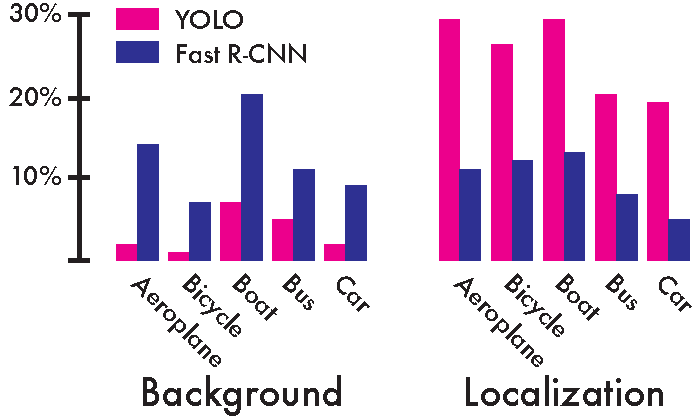
\includegraphics[width=\linewidth]{errors}
      \caption{\textbf{Error Analysis: Fast R-CNN vs. YOLO} These charts show the percentage of localization and background errors in the top N detections for various categories (N = \# objects in that category).}
      \label{errors}
   \end{wrapfigure}

Using the methodology and tools of Hoiem et al. \cite{hoiem2012diagnosing} we analyze our performance on the VOC 2007 test set. We compare YOLO to Fast R-CNN using VGG-16, one of the highest performing object detectors.

Figure \ref{errors} compares frequency of localization and background errors between Fast R-CNN and YOLO. A detection is considered a localization error if it overlaps a true positive in the image but by less than the required 50\% IOU. A detection is a background error if the box does not overlap any objects of any class in the image.

Fast R-CNN makes around the same number of localization errors and background errors. Over all 20 classes in the top N detections 13.6\% are localization errors and 8.6\% are background errors.

YOLO makes far more localization errors but relatively few background errors. Averaged across all classes, of its top N detections 24.7\% are localization errors and a mere 4.3\% are background errors. This is about twice the number of localization errors but half the number of background detections.

YOLO uses global context to evaluate detections while R-CNN only sees small portions of the image. Many of the background detections made by R-CNN are obviously not objects when shown in context. YOLO and R-CNN are good at different parts of object detection. Since their main sources of error are orthogonal, combining them should produce a model that is better across the board.

\subsection{Combining Fast R-CNN and YOLO}

YOLO makes far fewer background mistakes than Fast R-CNN. By using YOLO to eliminate background detections from Fast R-CNN we get a significant boost in performance. For every bounding box that R-CNN predicts we check to see if YOLO predicts a similar box. If it does, we give that prediction a boost based on the probability predicted by YOLO and the overlap between the two boxes. This reorders the detections to favor those predicted by both systems. Since we still use Fast R-CNN's bounding box predictions we do not introduce any localization error. Thus we take advantage of the best aspects of both systems.

\begin{table}[h]
\begin{center}
\begin{tabular}{lrrr}
 & mAP & Combined mAP & \% Pt Increase \\
\hline
Fast R-CNN & - & 71.8 & - \\
\hline
Fast R-CNN (2007 data) & 66.9 & 72.4 & .6  \\
Fast R-CNN (Small VGG) & 59.2 & 72.4 & .6 \\
Fast R-CNN (CaffeNet) & 57.1  & 72.1 &  .3\\
YOLO & 59.1  & 74.7 & 2.9\\
\end{tabular}
\end{center}
\caption{\textbf{Model combination expermients on VOC 2007.} We examine the effect of combining various models with the best version of Fast R-CNN. The model's base mAP is listed as well as its mAP when combined with the top model on VOC 2007. Other versions of Fast R-CNN provides only a small marginal benefit while combining with YOLO results in a significant performance boost.}
\label{combine}
\end{table}

The best Fast R-CNN model achieves a mAP of 71.8\% on the VOC 2007 test set. When combined with YOLO, its mAP increases by 2.9\% to 74.7\%. We also tried combining the top Fast R-CNN model with several other versions of Fast R-CNN. Those ensembles produced small increases in mAP between .3 and .6\%, see Table \ref{combine} for details. Thus, the benefit from combining Fast R-CNN with YOLO is unique, not a general property of combining models in this way.

Using this combination strategy we achieve a significant boost on the VOC 2012 and 2010 test sets as well, around 2\%. The combined Fast R-CNN + YOLO model performs on par with the best models on the VOC 2012 leaderboard.

\section{Conclusion}

We introduce YOLO, a unified pipeline for object detection. Our model is simple to construct and can be trained directly on full images. Unlike classifier-based approaches, YOLO is trained on a loss function that directly corresponds to detection performance and every piece of the pipeline can be trained jointly.

The network reasons about the entire image during inference which makes it less likely to predict background false positives than sliding window or proposal region detectors. Moreover, it predicts detections with only a single network evaluation, making it extremely fast.

YOLO achieves impressive performance on standard benchmarks considering it is 2-3 orders of magnitude faster than existing detection methods. It can also be used to rescore the bounding boxes produced by state-of-the-art methods like R-CNN for a significant boost in performance.

%A cell is only responsible for objects centered in that cell so we restrict the coordinates to fall within that cell. This imposes a strong spatial constraint on the predictions which has both benefits and drawbacks. Cells rarely predict multiple bounding boxes for the same object.

%Conversely, this spatial constraint limits the number of nearby objects that our model can predict. If two objects fall into the same cell our model can only predict one of them. Our model struggles with small objects that appear in groups, such as flocks of birds.

%Finally, our loss function treats errors the same in small bounding boxes versus large bounding boxes. A small error in a large box is generally benign but a small error in a small box has a much greater effect on IOU. Our main source of error is incorrect localizations.


{\small
\bibliographystyle{ieee}
\bibliography{egbib}
}

\end{document}
